\subsection{Connection time comparison} \label{sec:conn_time}

In this section of the analysis, we focus on connection time.
By connection time, we mean the time it takes for the underlying transport protocol to establish a secure connection.
For this analysis, we have not considered connection re-establishment.

Connection time is essential in IoT devices as many do not keep a connection alive while idling.
A device may opt not to be connected at all times to reduce energy consumption and computational power.
The device will then establish a connection and transmit data whenever required.
However, this means that some efficiency is lost if the connection has to be constantly re-established.
Hence, MQTT defines the period to keep the connection alive as the \textit{keep alive interval}.
In an MQTT/TCP implementation, the standard way to extend the keep alive interval is to periodically send a $ping$ packet, forcing the connection to remain open.
However, it has been shown that this method can lead to security vulnerabilities~\citep{vaccari_slowtt_2020,mileva_comprehensive_2021}.

To measure the connection time, we have followed the previously described methodology.
That is, we began a communication via MQuicTT and the other MQTT implementations and captured it using $tcpdump$.
We have then extracted the time between the start of the QUIC or TCP communication and the handshake completion.

Figure~\ref{fig:connect_time_home} shows the results for the IoT home scenario.
We can see that $MQuicTT$ connects fractionally slower than the base implementation across the links on average, with the least overlap being on 3g and 4g links.
However, when factoring in the variance, both implementations perform equally well.
Notably, $MQuicTT$ shows higher variance in connection time, while the TCP implementation is consistent.
This result can be attributed to the fact that QUIC's advantage comes in scenarios with packets loss and the IoT home scenario does not implement high packet loss.
QUIC should still theoretically connect faster due to its simpler handshake, however, the implementation may impose overhead that outweighs this.

\begin{figure}
    \centering
    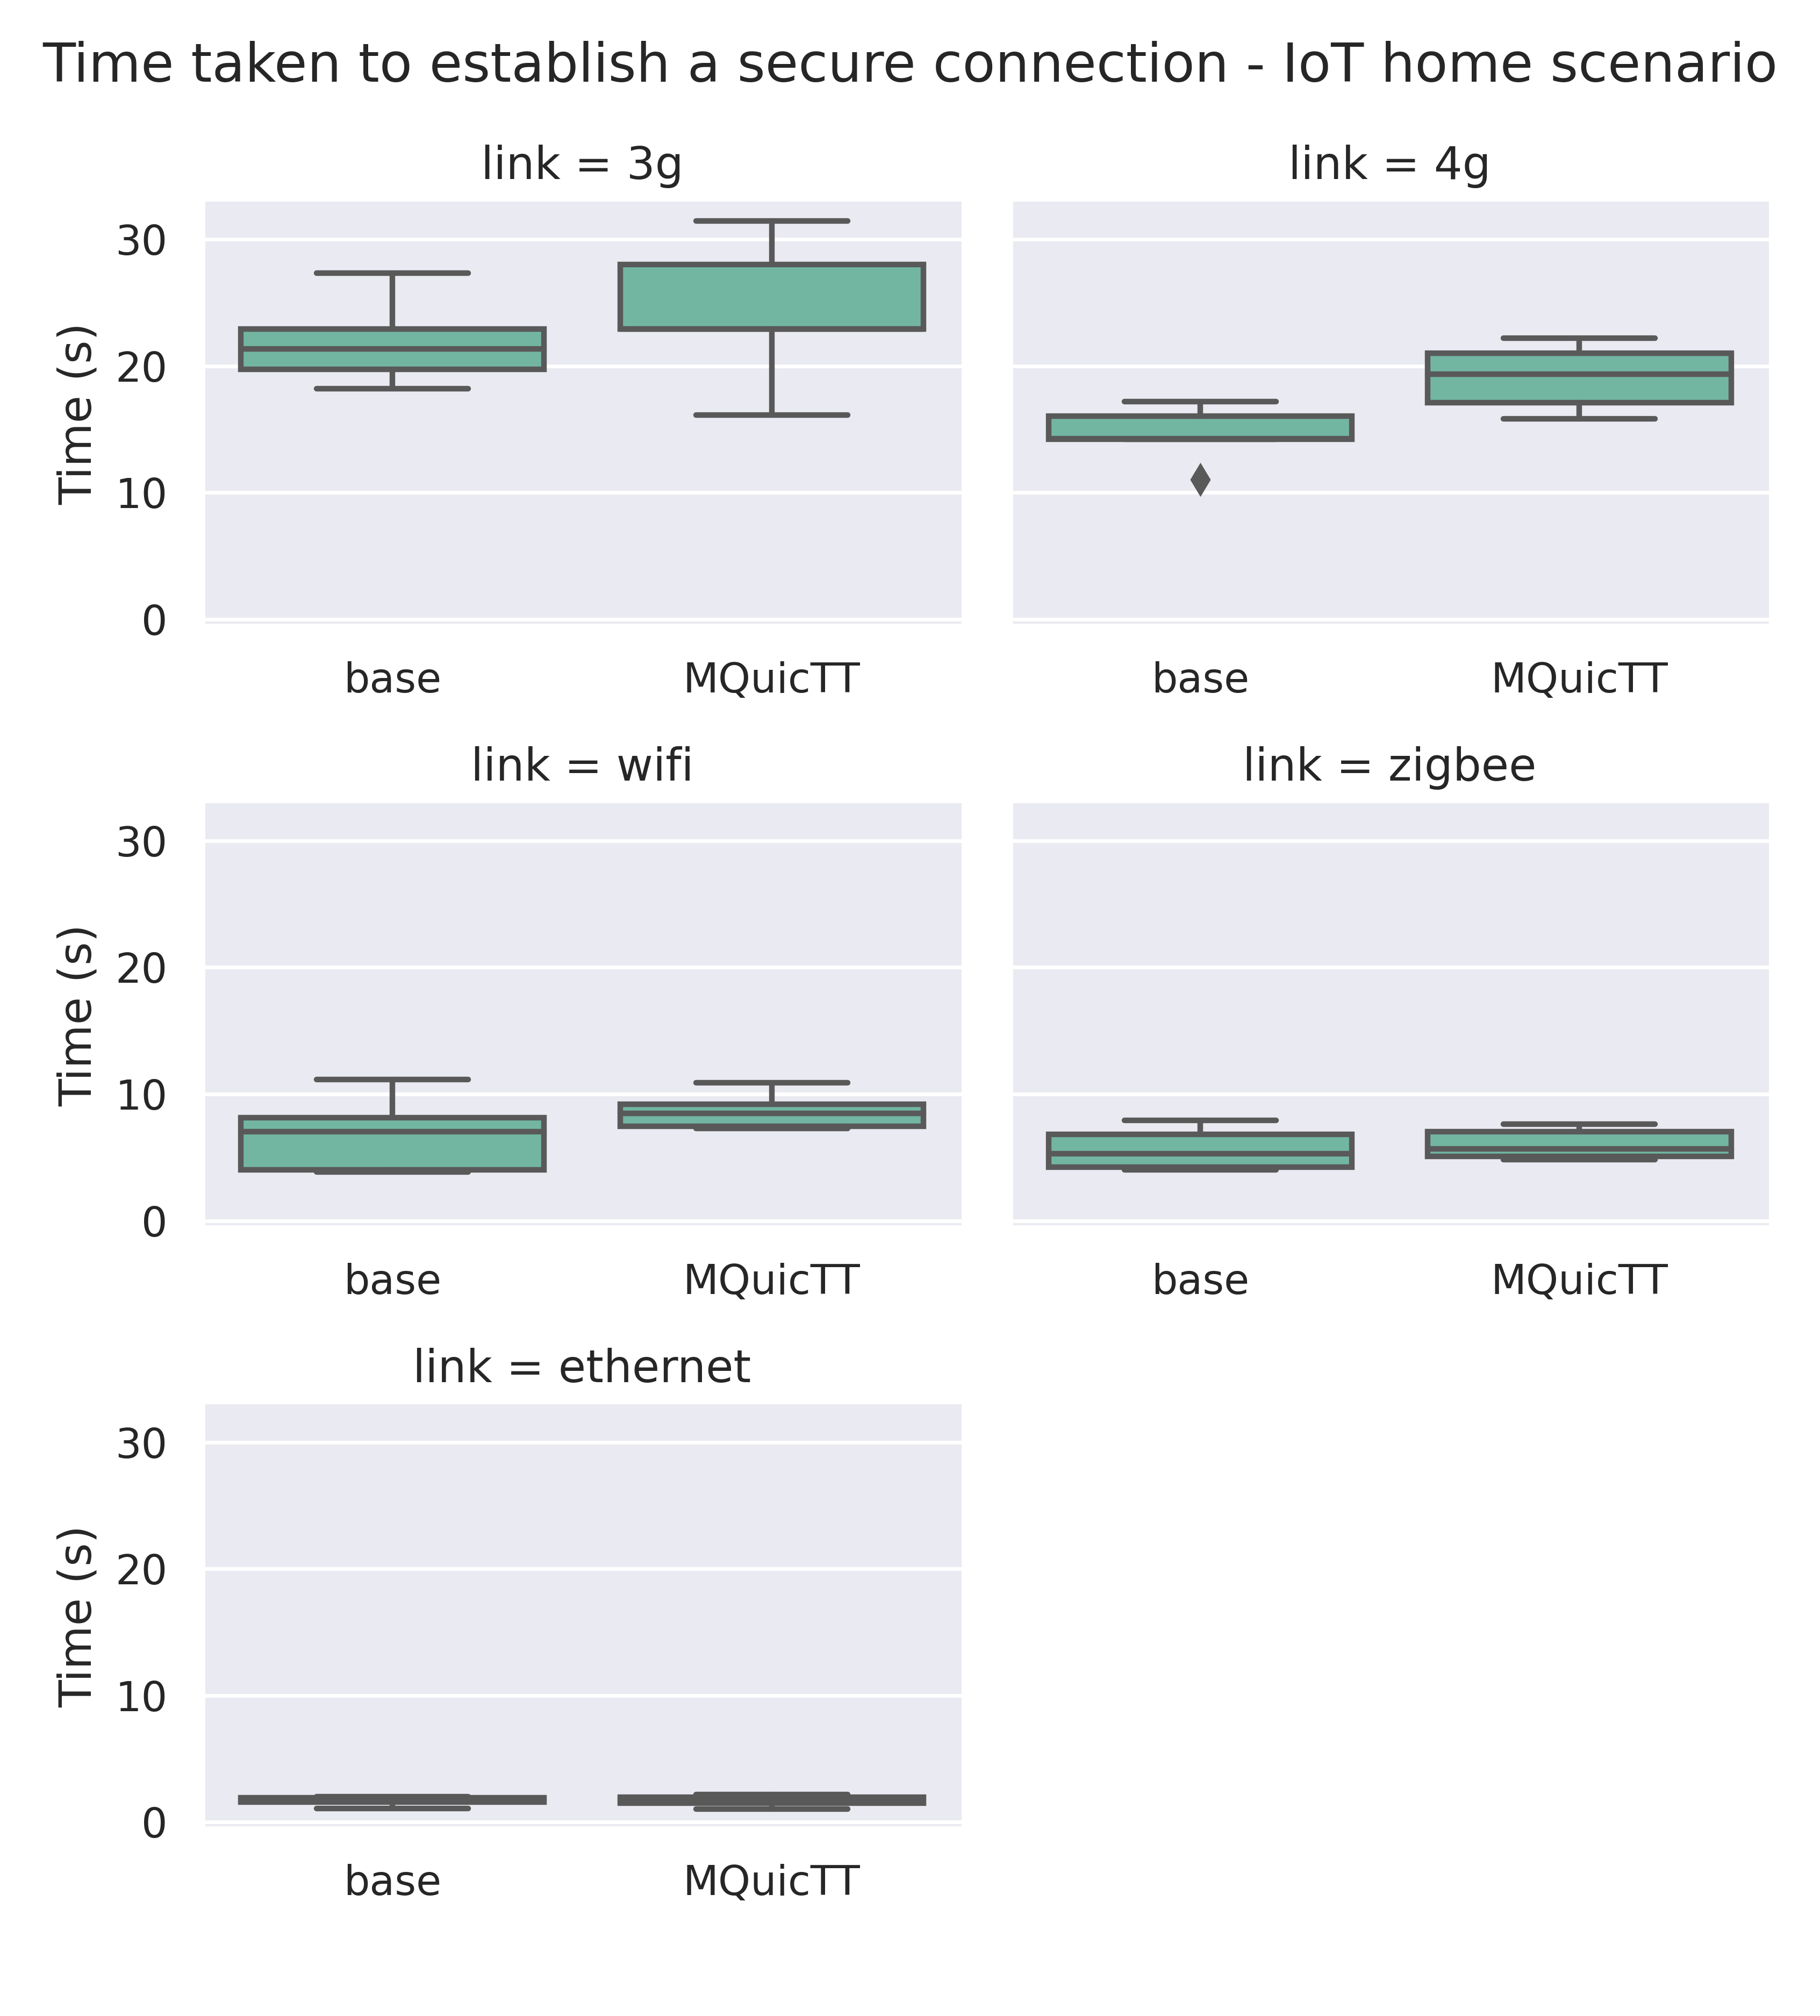
\includegraphics[width=1\linewidth]{images/analysis_connection_time_home.png}
    \caption{The time it took for the implementations to establish a secure connection in the IoT home scenario for each link.
        We can see that MQuicTT experiences higher variance, but performs on par with the base implementation overall.}
    \label{fig:connect_time_home}
\end{figure}


On the other hand, in the printer farm scenario, as shown in Figure~\ref{fig:connect_time_farm}, we can see that $MQuicTT$, on average, establishes a connection faster than the base implementation.
We can see that, accounting for variance, the performance advantage is approximately on the scale of a single round trip time.
This is consistent with the assumption that QUIC can handle packet loss better than the base TCP implementation.
That is, the QUIC implementation likely did not need to retransmit packets as much as the base implementation, hence establishing a quicker connection.

\begin{figure}
    \centering
    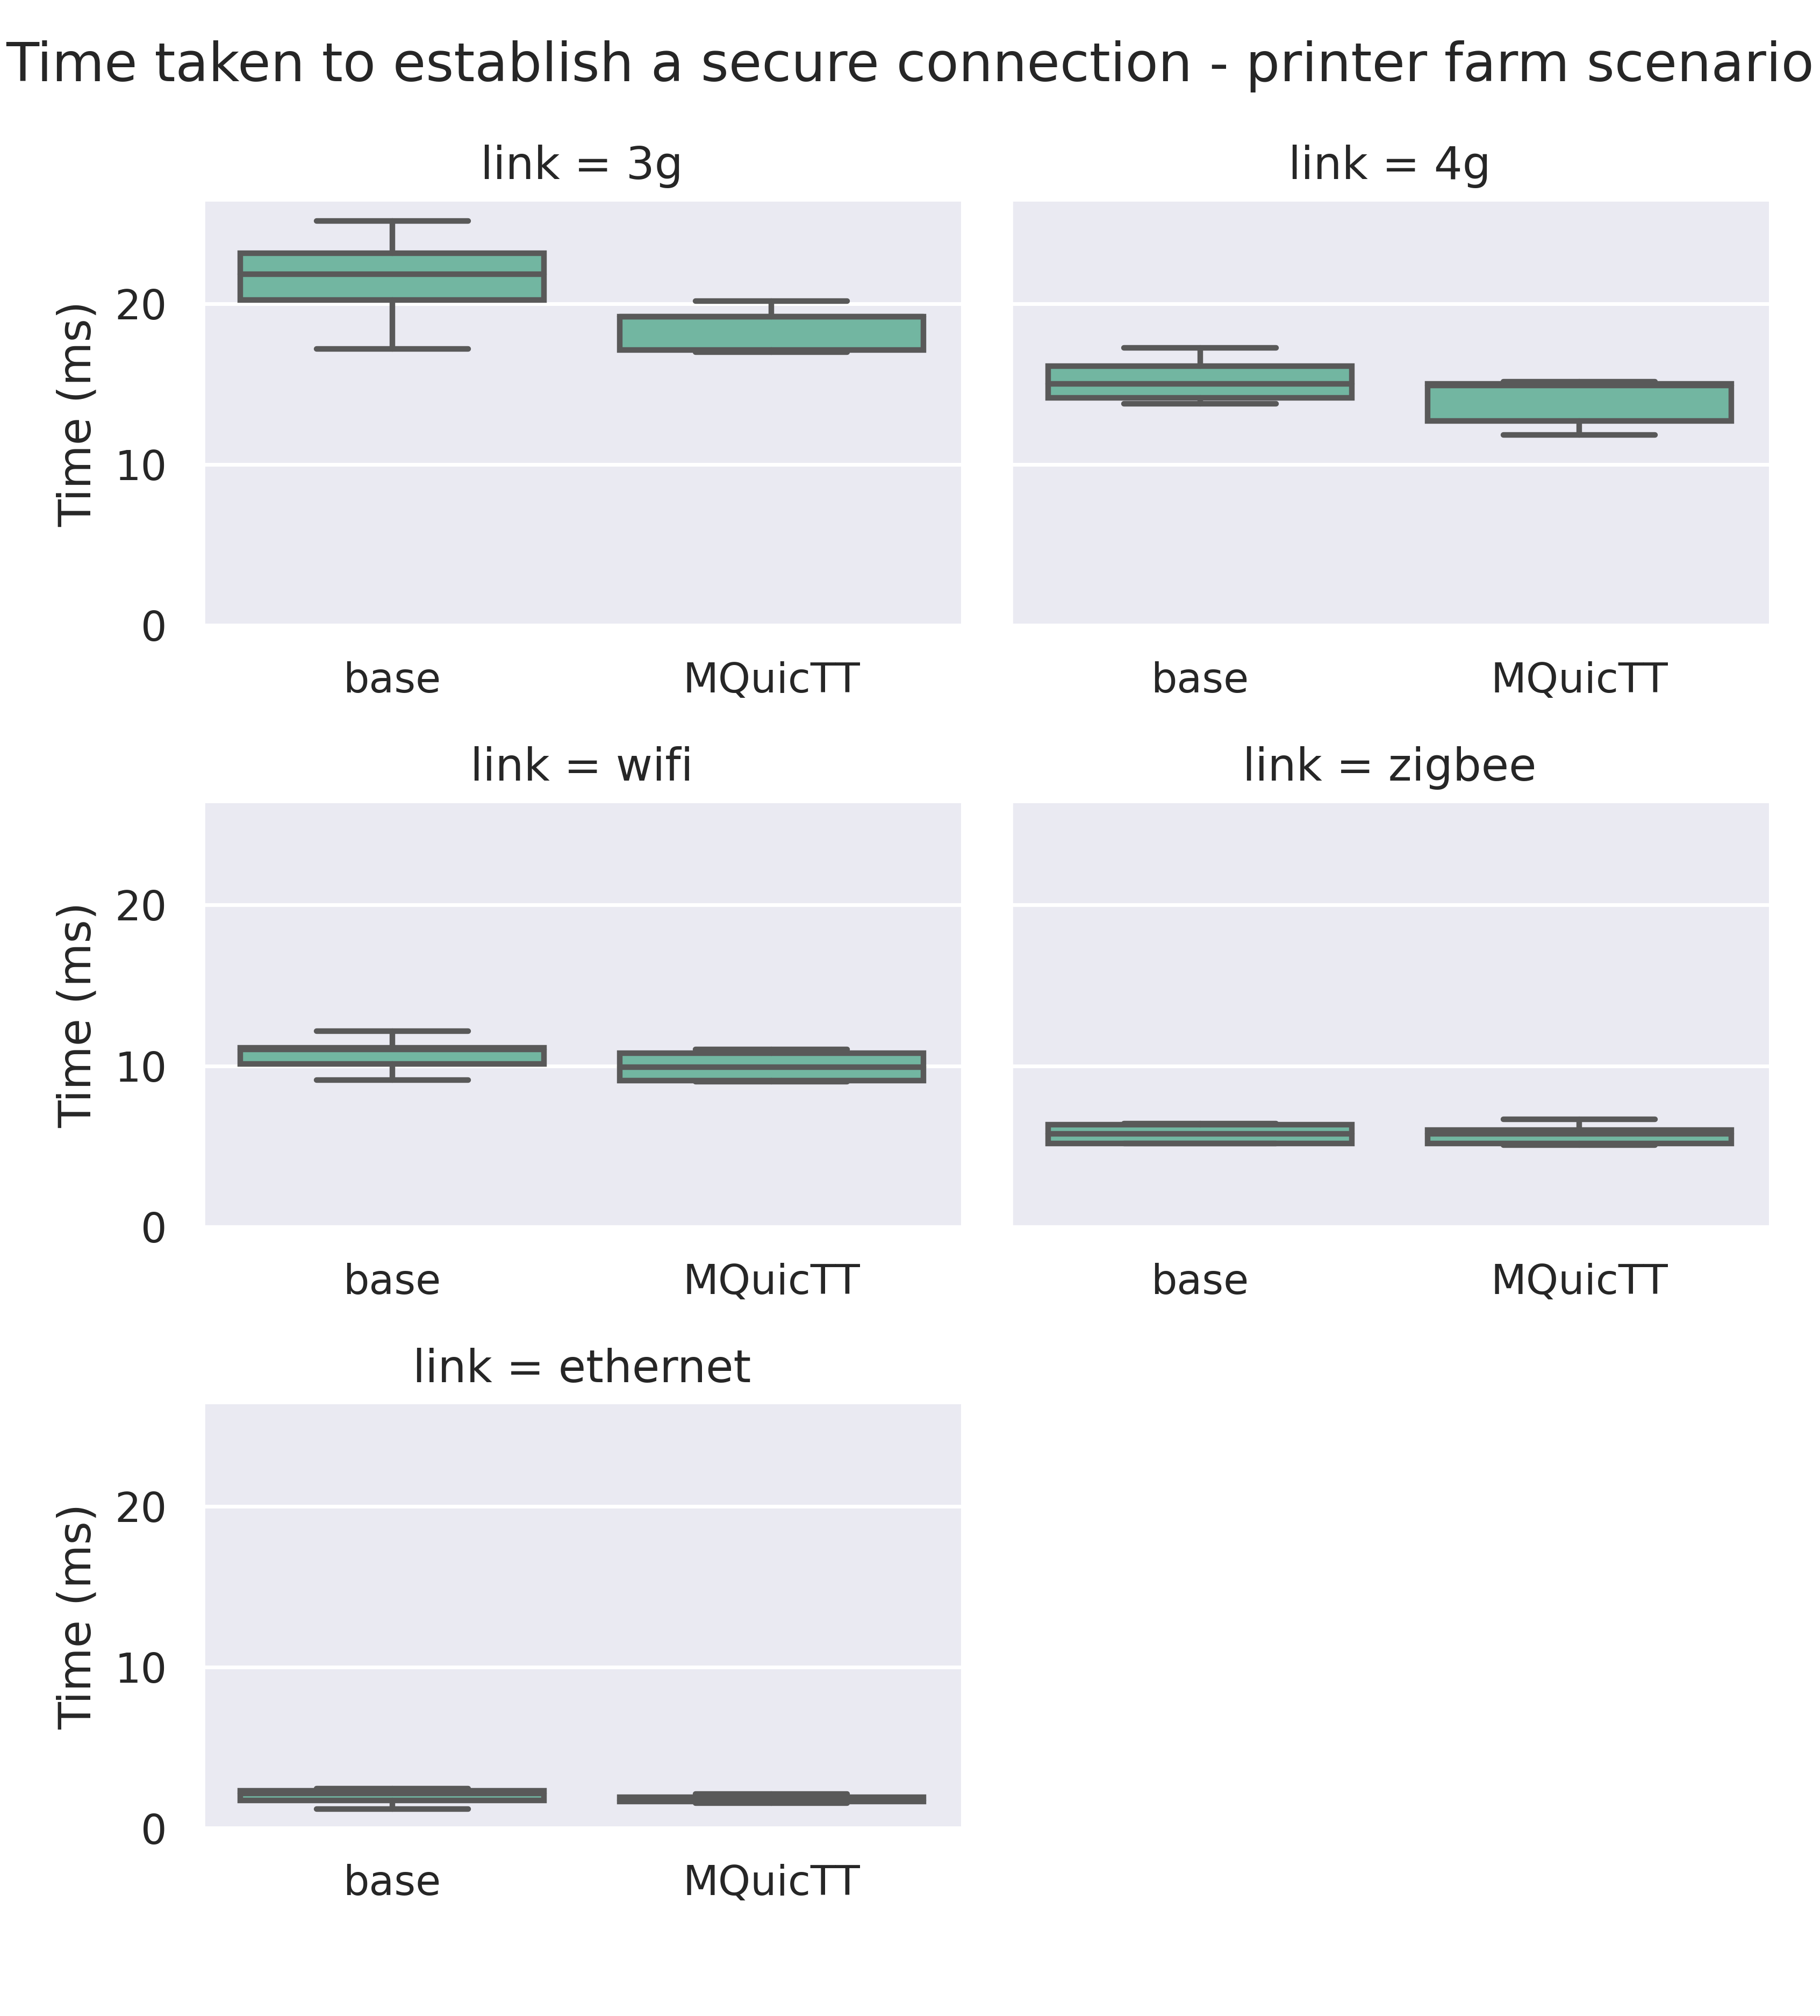
\includegraphics[width=1\linewidth]{images/analysis_connection_time_farm.png}
    \caption{The time it took for the implementations to establish a secure connection in the printer farm scenario for each link.
        We can see that MQuicTT experiences higher variance, but performs on par with the base implementation overall.}
    \label{fig:connect_time_farm}
\end{figure}

\begin{figure}
    \centering
    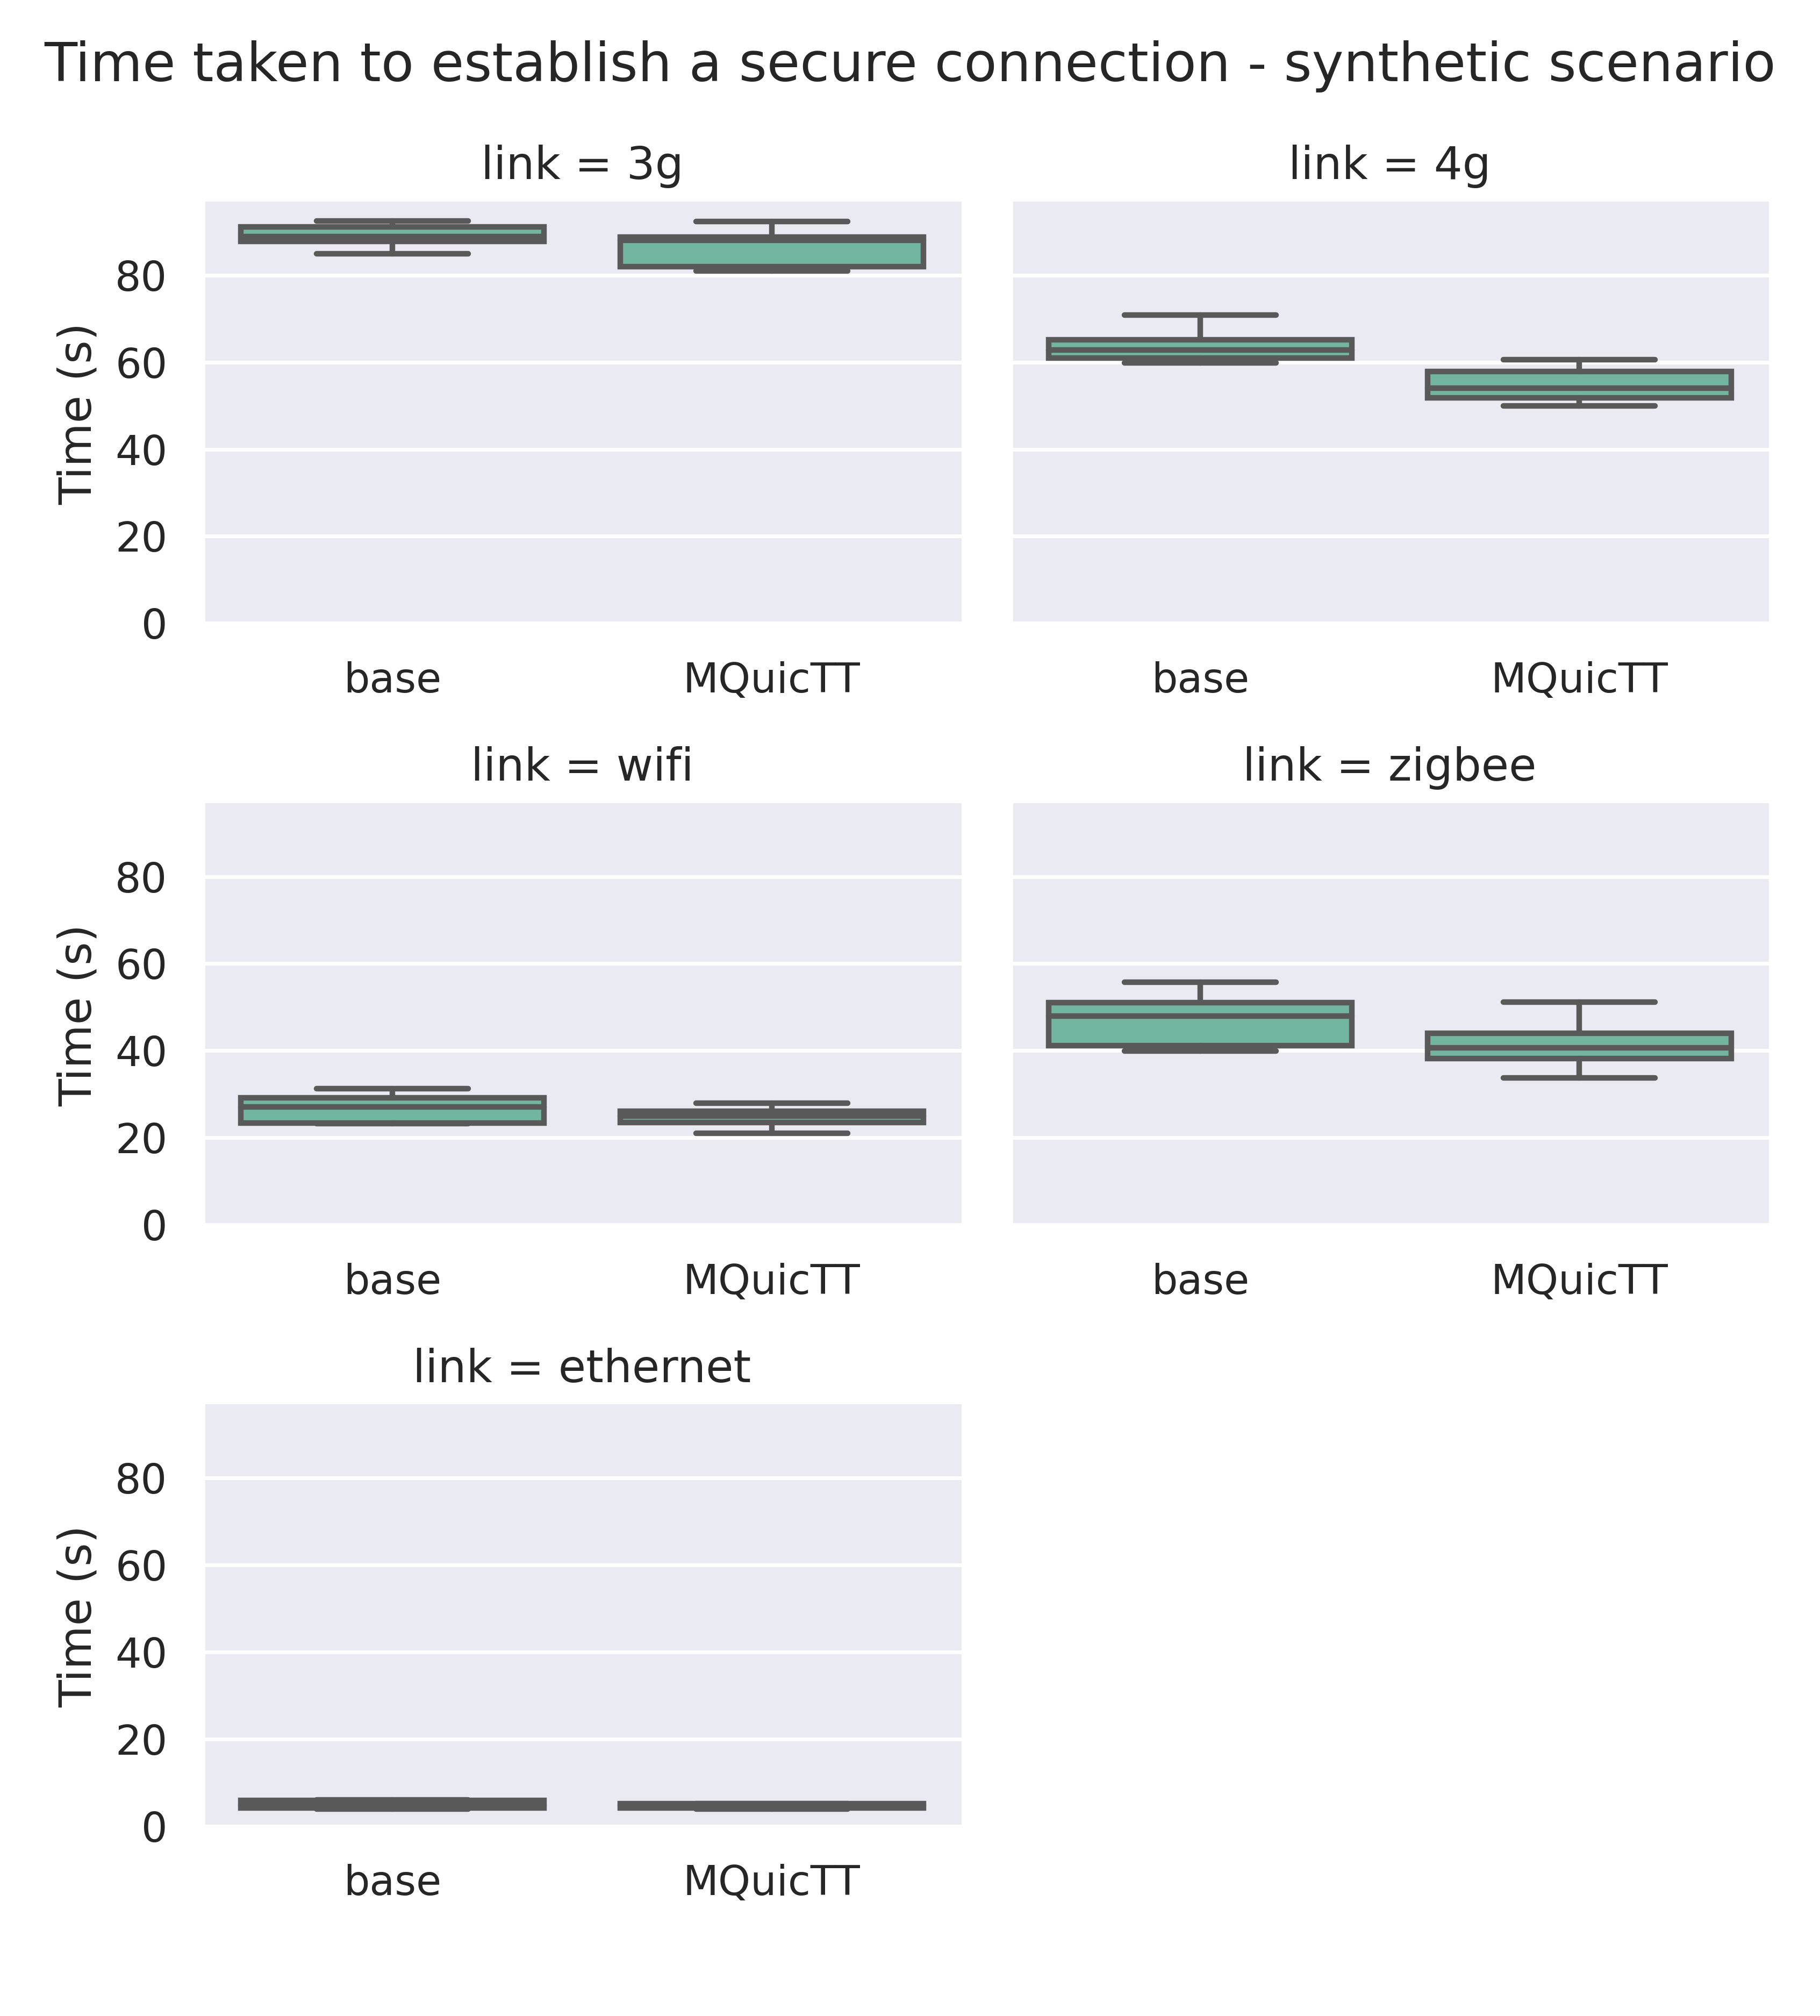
\includegraphics[width=1\linewidth]{images/analysis_connection_time_synth.png}
    \caption{The time it took for the implementations to establish a secure connection in the printer farm scenario for each link.
        We can see that MQuicTT experiences higher variance, but performs on par with the base implementation overall.}
    \label{fig:connect_time_synth}
\end{figure}

This result is supported by the data obtained from the synthetic scenario shown in Figure~\ref{fig:connect_time_synth}.
We can see that $MQuicTT$ again, on average, establishes a connection quicker than the base implementation.
This is expected as the packet loss here is extreme, hence, QUIC should perform better on average.


Overall, $MQuicTT$ presents an advantage in terms of time needed to establish a connection in environments with high packet loss, however, is not advantageous for the IoT home scenario.
These results support some of the theoretical advantages of QUIC, however, they also show that the advantage may not be as high as reported in the literature.